\documentclass[12pt]{article}
\usepackage[a4paper, total={7in, 9in}]{geometry}

\usepackage{lipsum}
\usepackage{epsfig}
\usepackage[labelformat=simple]{subcaption}

\renewcommand\thesubfigure{\alph{subfigure}}
\DeclareCaptionLabelFormat{subcaptionlabel}{\normalfont(\textbf{#2}\normalfont)}
\captionsetup[subfigure]{labelformat=subcaptionlabel}


\usepackage{listings}
\usepackage{xcolor}

\lstset{
    numbers=left,
    breaklines=true,
    backgroundcolor=\color{lightgray},
    tabsize=2,
    basicstyle=\ttfamily,
    literate={\ \ }{{\ }}1
}

\title{Using PyAutoLens for Generation of Adversial Examples for a Convolutional Neural Network Model}


\author{Mohammed Asfour}       


\setlength{\parskip}{6pt}

\begin{document}
\maketitle

\abstract% 
Software for astronomy has had great advances in the previous year to ease the processing and exploration of space phenomena. Such an example is the generation of an image of the black hole in 2019. This report outlines the usage of one of such packages called PyAutoLens. PyAutoLens is a python package for gravitational lens problems, which can be summarized by the bending of the light travelling across the galaxy. The light can bend due to the mass of nearby galaxies or even black holes, which prohibits us from reaching a clear visualization from distant stars past our solar system. The proposed package in this report uses PyAutoLens to generate synthesized images of the gravitational lens phenomenon, and trains a convolutional neural network (CNN) to train on raw images from space telescopes to predict properties of the distant starts to better understand them from their bent light.

% \setcounter{tocdepth}{0}
\section{Introduction}
Astronomical phenomena has been throughly explored\cite{astro5}\cite{astro3}\cite{astro4}; yet, it's the trend to use newly released packages for model fitting to explain such phenomena\cite{astro1}\cite{astro2}.
Gravitational Lens is the name given to the phenomenon of bending the lights of stars while travelling past bodies with significant gravitational pull. It's common to call the distant source of the bent light by "source galaxy", while the galaxy with the significant gravitational pull as "lens galaxy". Due to that phenomenon, space telescopes could produce images of distant galaxies or starts that are warped, resulting into straight beams of light to be seen as a circle or a curve. An illustration of this can be seen in Fig. \ref{fig:grav}

The problem of gravitaional lens is solved using ray tracing. By knowing more about the source galaxy and the lens galaxy, we can simulate how the light is bent while travelling to reach the exact point it had reached in the space telescope image. The ray tracing can then be used to know the real source galaxy.


\begin{figure}[thb]
    \centering
    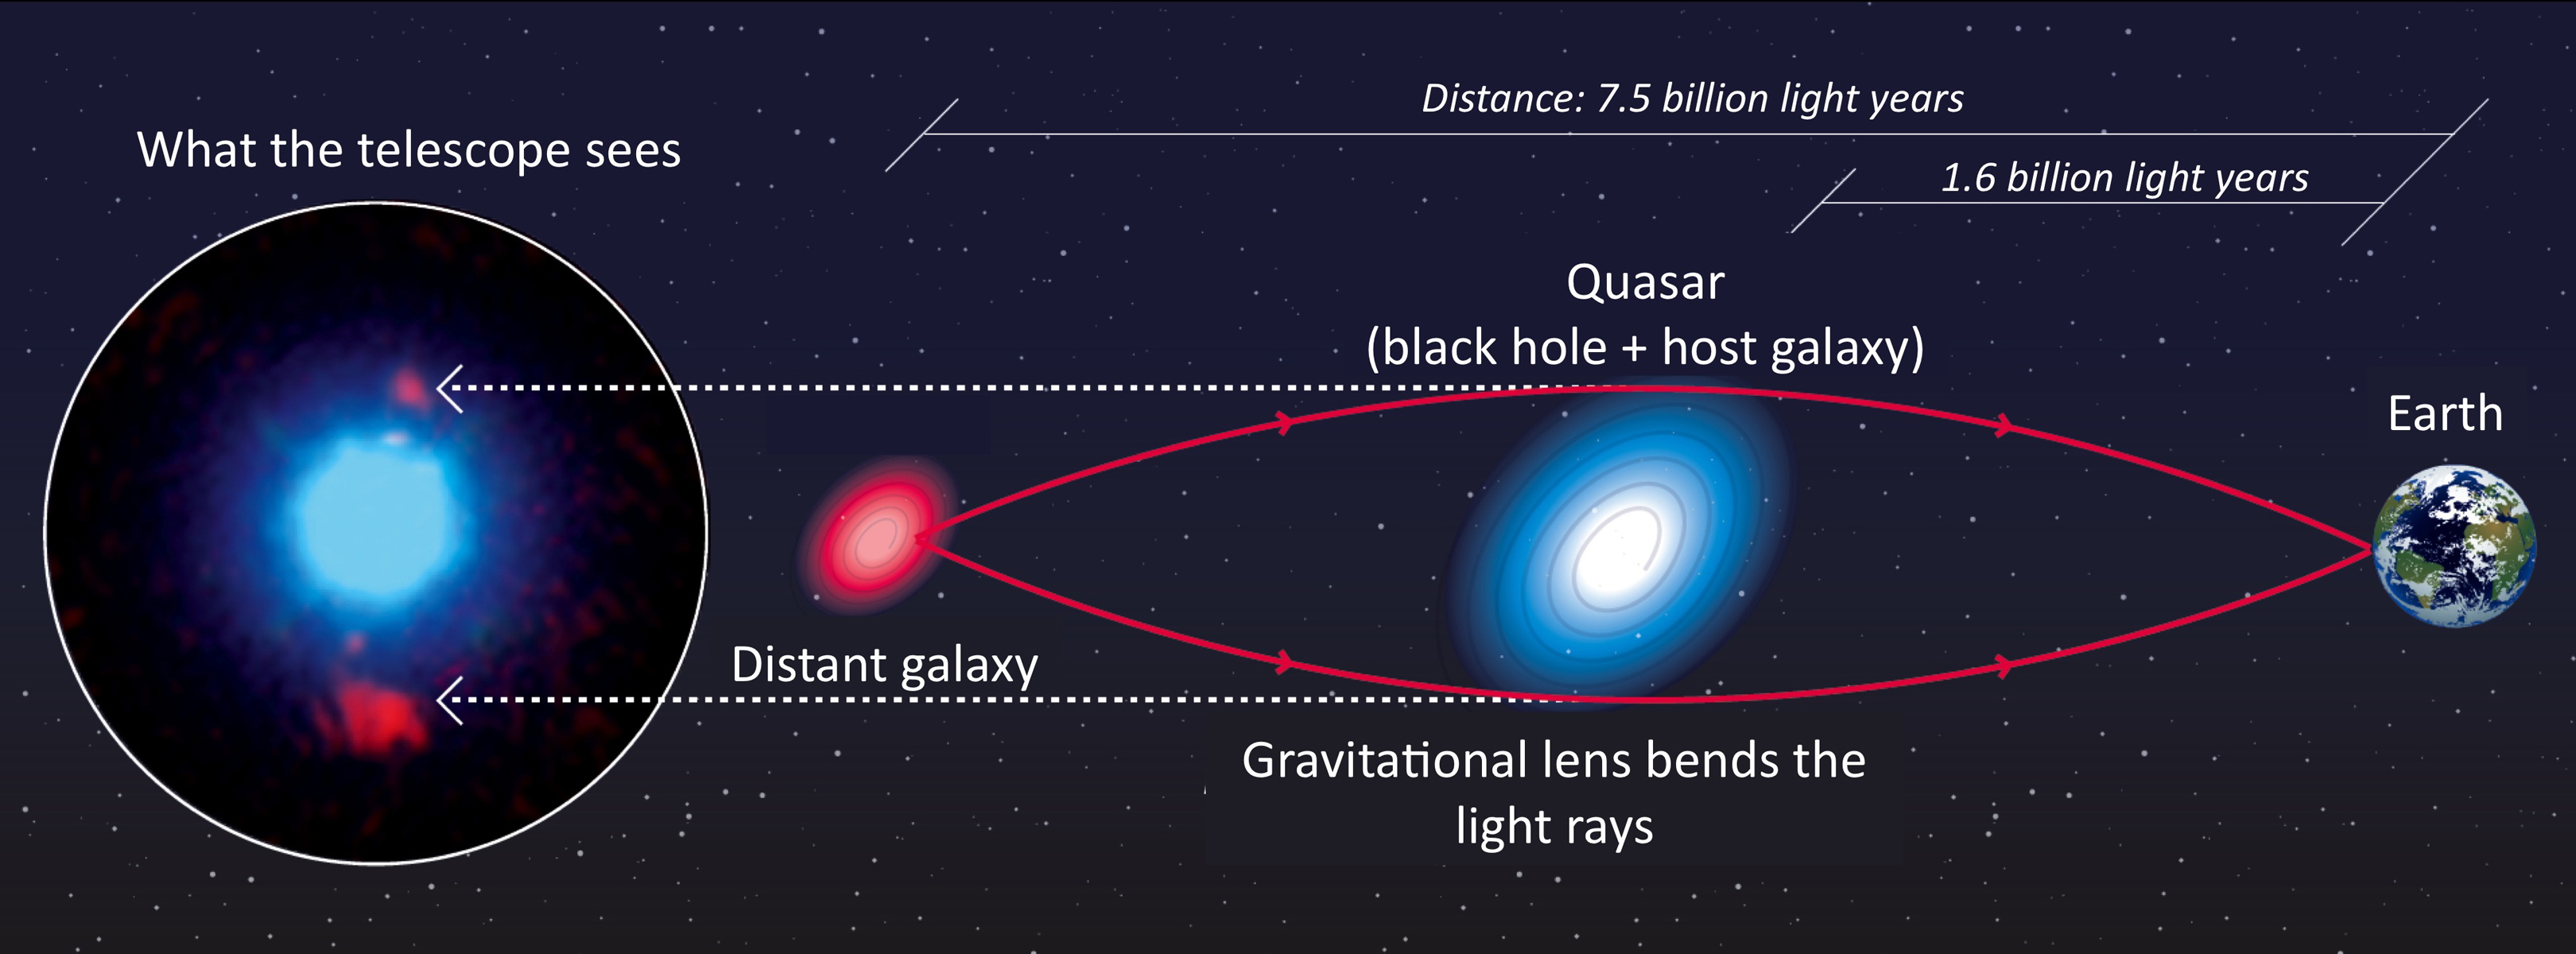
\includegraphics[width=\textwidth]{grav_lens.jpeg}
    Image credit: F. Courbin, S. G. Djorgovski, G. Meylan, et al., Caltech / EPFL / WMKO
    \caption{An Example of the Gravitational Lens Phenomenon.}
    \label{fig:grav}
\end{figure}


\section{Methodology}
\subsection{Scripts}
\subsubsection{params\_and\_cli.py}
This script is responsible for holding on the hyper-parameters that will control the generation of the dataset, training of the model, and producing the figures.
\newline\newline
It contains the hyper-parameters values, as well as the command line interface (CLI) arguments, their description, and their shortcuts. On top of that, it contains the functions that parse the cli passed arguments and modifies the behavior of other scripts. Lastly it includes the functions and information necessary to print out a help table for each of the other two file to the cli using the argument --help while running the other two scripts.

\subsubsection{generate\_data.py}
This script is used to randomly generate gravitational lens problem settings using hyperparameters, and saves the generated results as .pickle files in ./dataset with a csv file containing the labels (properties of the source
galaxy)

It contains functions that use samples generated from "params\_and\_cli.py" script to produce the gravitational lens example solve the ray tracing problem and produce the final image that would have been taken by a telescope as an array. The array is then saved as a ".pickle" intermediate file to be used for more processing.

The following code can be run in the cli to use the script

\begin{lstlisting}[mathescape=true, language=python]
The hyperparameters controlling the generation process can be set using the cli arguments while running the script.
    For example:
        $ \color{blue}
            python\ generate\_data.py\ --src-intensity-range=0.3,1.0
        $
        
To view all the possible arguments and their description use:
        $ \color{blue}
            python\ generate\_data.py\ --help
		$
\end{lstlisting}

\subsubsection{model\_and\_figures.py}
This script creates a TensorFlow CNN model using a pre-defined architecture. The script then trains the models, and saves it followed by producing figures locally.

This script contains does of the work of the proposed package as it has to train a convolution model, and produce activation figures of the convolutional layers which could be a bit computationally extensive.

The following code can be run in the cli to use the script

\begin{lstlisting}[mathescape=true, language=python]
The hyperparameters controlling the training and figures can be set using the cli arguments while running the script.
    For example:
        $ \color{blue}
            python\ model\_and\_figures.py\ --epochs=50\ -f=png
        $
        
To view all the possible arguments and their description use:
        $ \color{blue}
            python\ model\_and\_figures.py\ --help
		$
\end{lstlisting}

\subsection{Model Architecture}
Using a convolutional neural network, the package is able to leverage the deep learning power to learn patterns from images and predict properties of the source galaxy.

The model used is a sequential model, meaning each layer is feeding into the one after it. The whole architecture has a total of 1,214,307 parameters with layers output shapes as follows in Table \ref{tab:nn_param}


\begin{itemize}
    \item Input Layer (None, 64, 64, 1)
    \item 2D Convolution (None, 64, 64, 32)
    \item Pooling (None, 32, 32, 32)
    \item 2D Convolution (None, 32, 32, 64)
    \item Pooling (None, 16, 16, 64)
    \item 2D Convolution (None, 16, 16, 128)
    \item Pooling (None, 8, 8, 128)
    \item flatten (None, 8192)
    \item Fully-Connected (None, 128)
    \item Dropout (None, 128)
    \item Fully-Connected (None, 3)
\end{itemize}

The following hyper-parameters were used for training

\begin{table}
    \centering
    \begin{tabular}{c|c}
        
        \textbf{Hyperparameter} & \textbf{Default Value} \\
        
        valid-split & 0.2 \\
        test-split & 0.1 \\
        labels & src-redshift, src-center-x, src-center-y \\
        epochs & 50 \\
        learning-rate & 0.00001 \\
        batch-size & 20 \\
    \end{tabular}
    \caption{Hyperparameters used in model training}
    \label{tab:nn_param}
\end{table}

\subsection{Figures}
The figures to be produced will be split into 3 distinguished categories:
\begin{itemize}
    \item Visualization of the samples generated by the PyAutoLens\cite{pyautolens} package
    \item The losses curves of the training of the neural network
    \item The visualization of convolutional layer activations.
\end{itemize}

\section{Results}
\subsection{The Generated Samples}
Firstly we visualize the gravitaional lens adversial examples generated by the PyAutoLens\cite{pyautolens} packge. Examples of the samples can be seen in Fig. \ref{fig:samples}


\begin{figure}[thb]
    \centering
    
    \begin{minipage}{\columnwidth}
	\begin{subfigure}{0.5\columnwidth}
    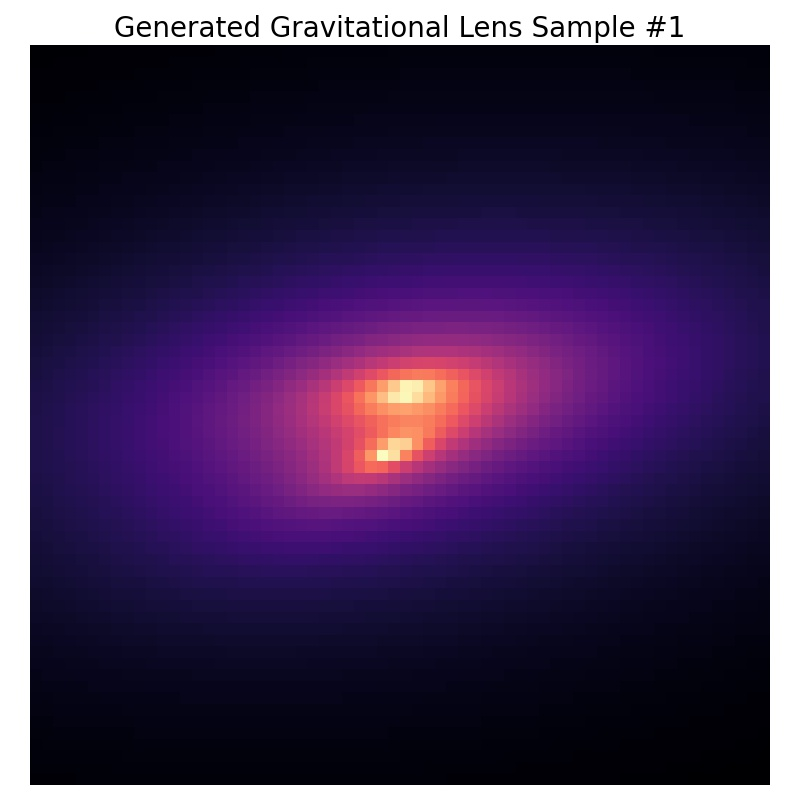
\includegraphics[width=\columnwidth]{../figures/img1.jpg}
    % \vspace*{-15pt}
    \caption{}
    \label{fig:sample1}
    \end{subfigure}
    \begin{subfigure}{0.5\columnwidth}
    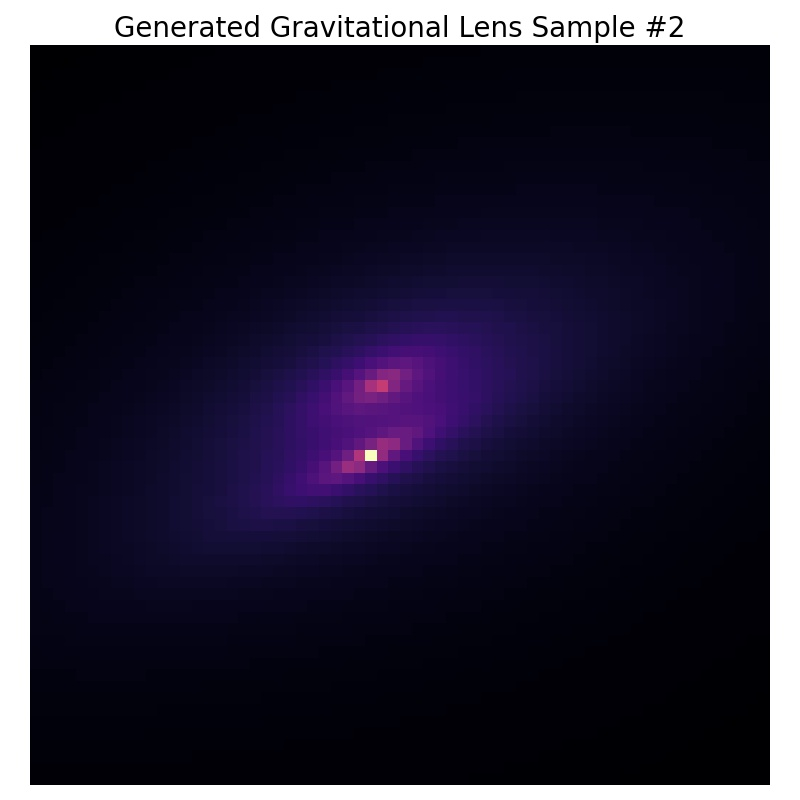
\includegraphics[width=\columnwidth]{../figures/img2.jpg}
    % \vspace*{-15pt}
    \caption{}
    \label{fig:sample2}
    \end{subfigure}
\end{minipage}

\begin{minipage}{\columnwidth}
	\begin{subfigure}{0.5\columnwidth}
    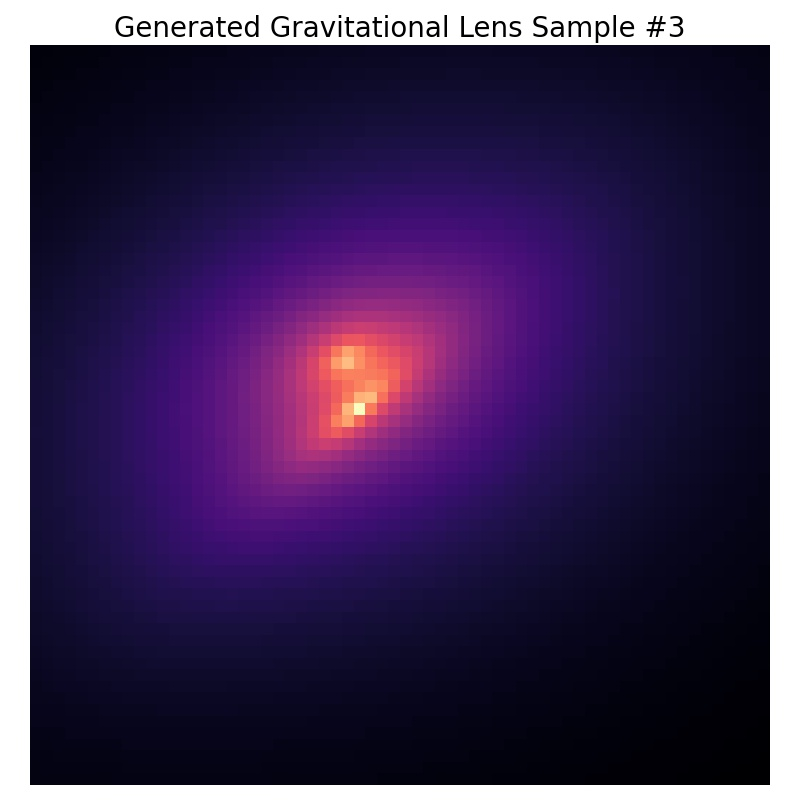
\includegraphics[width=\columnwidth]{../figures/img3.jpg}
    % \vspace*{-15pt}
    \caption{}
    \label{fig:sample3}
    \end{subfigure}
    \begin{subfigure}{0.5\columnwidth}
    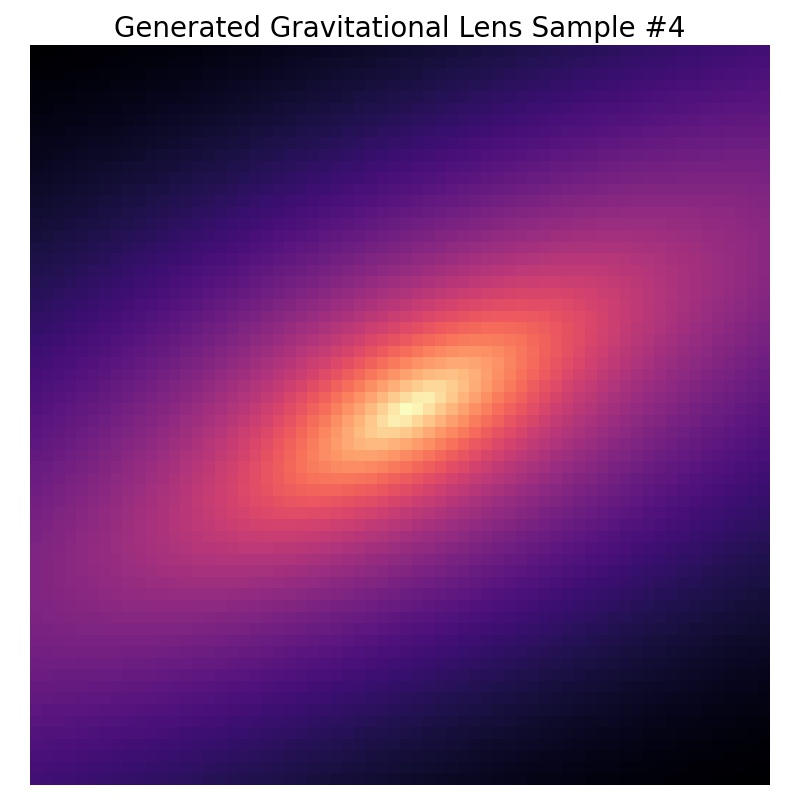
\includegraphics[width=\columnwidth]{../figures/img4.jpg}
    % \vspace*{-15pt}
    \caption{}
    \label{fig:sapmle4}
    \end{subfigure}
\end{minipage}

    \caption{Visualization of samples generated by PyAutoLens\cite{pyautolens} of the gravitational lens phenomenon.}
    \label{fig:samples}
\end{figure}

\subsection{Model Training}
We can then feed the sampled images with the samples properties to train the model, resulting in the following loss curves in Fig. \ref{fig:loss}


\begin{figure}[thb]
    \centering
    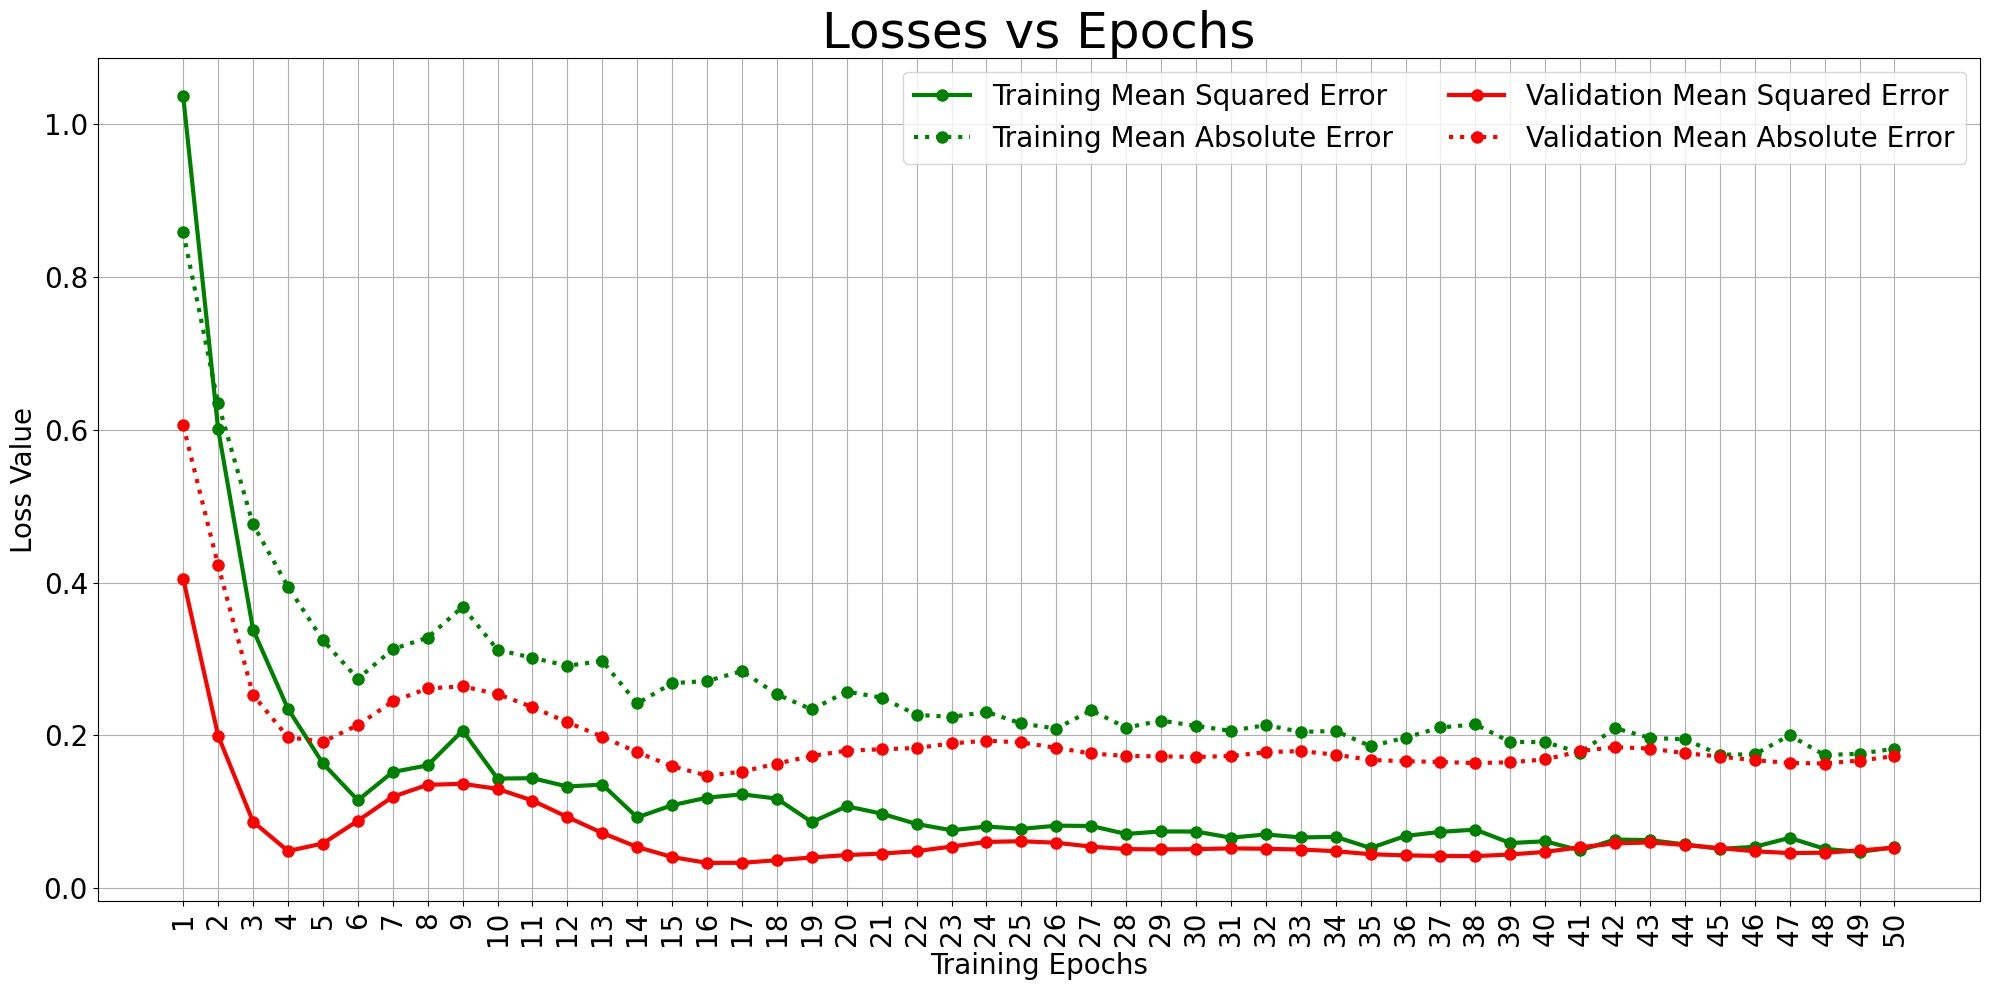
\includegraphics[width=\textwidth]{../figures/loss_epochs.jpg}
    \caption{The training and validation losses of the model during training}
    \label{fig:loss}
\end{figure}


\subsection{Visualization of Convolutinal Layers Activations}
Finally we are able to visualize the activations of the convolutional layers in the model to better understand which characteristics of the images that the model use to predict the properties of the source galaxy. The input image to the model can be seen in Fig. \ref{fig:conv_inp}, while the activations of the convolutional layers are reported in Fig. \ref{fig:conv1}, Fig. \ref{fig:conv2}, and Fig. \ref{fig:conv3}.

\begin{figure}[thb]
    \centering
    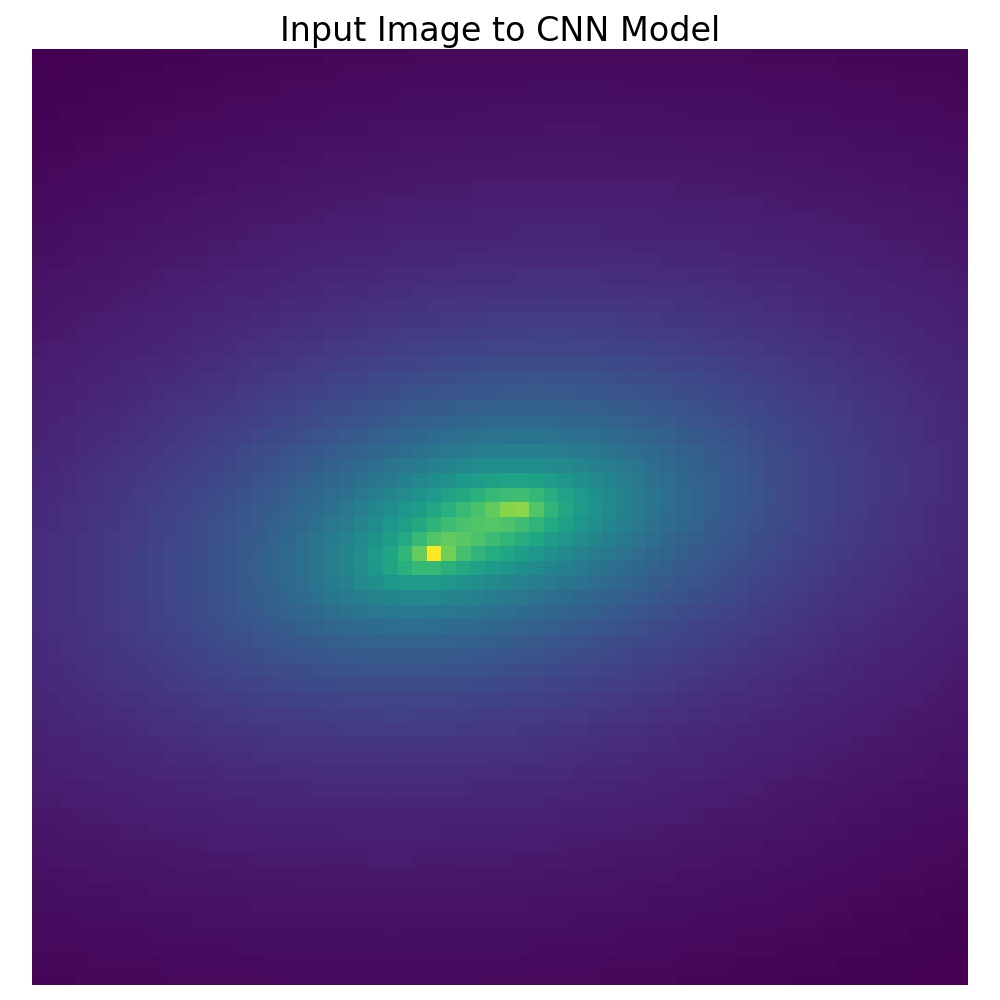
\includegraphics[width=\textwidth]{../figures/conv_input.jpg}
    \caption{Input image to the CNN model generated by PyAutoLens\cite{pyautolens} package}
    \label{fig:conv_inp}
\end{figure}

\begin{figure}[thb]
    \centering
    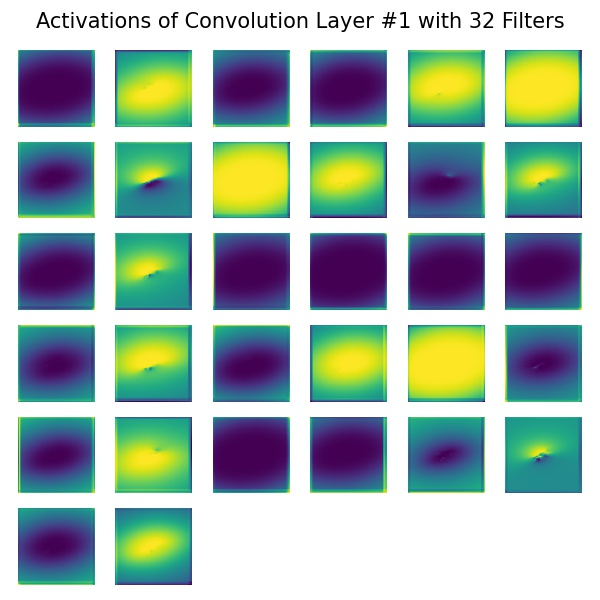
\includegraphics[width=\textwidth]{../figures/conv_activ1.jpg}
    \caption{Activation of the filters of the first convolutional layer corresponding to the sample image generated by PyAutoLens\cite{pyautolens} package}
    \label{fig:conv1}
\end{figure}

\begin{figure}[thb]
    \centering
    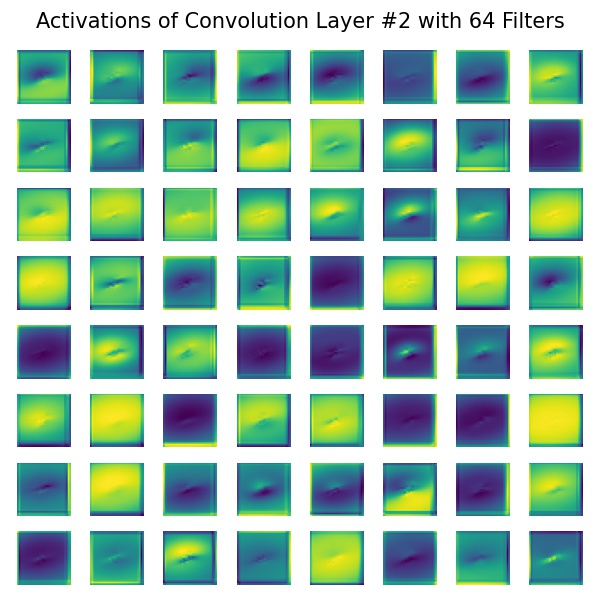
\includegraphics[width=\textwidth]{../figures/conv_activ2.jpg}
    \caption{Activation of the filters of the second convolutional layer corresponding to the sample image generated by PyAutoLens\cite{pyautolens} package}
    \label{fig:conv2}
\end{figure}

\begin{figure}[thb]
    \centering
    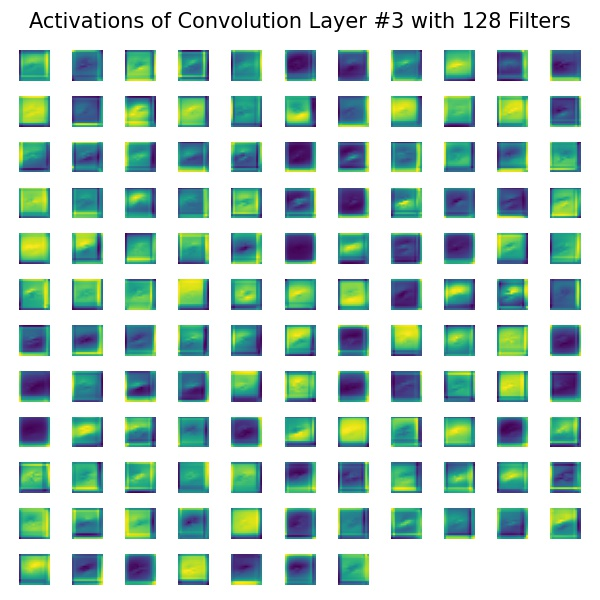
\includegraphics[width=\textwidth]{../figures/conv_activ3.jpg}
    \caption{Activation of the filters of the third convolutional layer corresponding to the sample image generated by PyAutoLens\cite{pyautolens} package}
    \label{fig:conv3}
\end{figure}

\clearpage
\bibliographystyle{ieeetr}
\bibliography{ref}  
\end{document}
